\documentclass[fontsize=28pt,a4paper]{scrartcl}

\usepackage[margin=0.75in,includefoot,bottom=0.3in,footskip=2em]{geometry}

\usepackage{fontspec}
\setmainfont{EBGaramond}
[
  Extension      = .otf ,
  UprightFont    = *-Regular,
  ItalicFont     = *-Italic,
  BoldFont       = *-Bold,
  BoldItalicFont = *-BoldItalic,
  Numbers        = Lowercase,
  Ligatures      = Discretionary,
  Style          = Swash
]
% https://texnique.fr/osqa/questions/8423/lualatex-et-ligatures

\usepackage[french]{babel}

% https://tex.stackexchange.com/a/123669/295527
%\renewcommand*{\FrenchLabelItem}{$\bullet$}
%\frenchsetup{StandardItemLabels=true}
\frenchsetup{StandardLayout=true}

\usepackage{microtype}

\usepackage{xcolor}
\usepackage{tikz}
\usetikzlibrary{intersections,calc}
\usepackage{caption}
\usepackage{longtable,booktabs,array}
\usepackage{comment}

\usepackage[showmarks]{pocketmod}% https://github.com/liantze/pocketmod.sty

% https://fr.overleaf.com/latex/examples/mini-livre-trigonometrie/ntgbdvthxhnb
% https://fr.overleaf.com/latex/examples/mini-livre-exercices-de-rentree-en-seconde/gncxgskzswtc
% https://forge.apps.education.fr/duplessyerwan/site-mini-math-livre

\usepackage{graphicx}
\usepackage{enumitem}
\setlist{leftmargin=\parindent,labelindent=*}
\usepackage{hyperref}
\usepackage[hyphenbreaks]{breakurl}

%\title{Creating PocketMods with \LaTeX}
\title{Socrate et la rhétorique}

%\author{LianTze Lim}
%\author{\small Vincent Pantaloni}
\author{\small R. Chastain}
\date{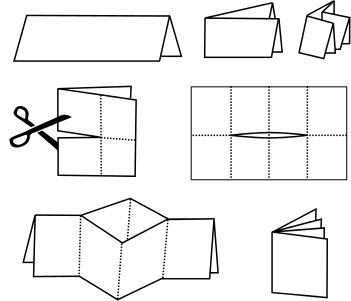
\includegraphics[width=.75\textwidth]{folding-minibook}}

\begin{document}

\thispagestyle{empty}
\maketitle

\clearpage

\subsection*{La nature de la rhétorique selon Gorgias}

%Gorgias est de passage à Athènes, pour y donner une conférence. Il invite l'auditoire à lui poser n'importe quelle question, à laquelle il promet de répondre par un discours improvisé. 

Socrate interroge Gorgias sur \emph{ce qu'il est} : il voudrait connaître le nom et la nature de l'art que Gorgias enseigne.

Cet art, c'est la rhétorique. C'est l'art de persuader des citoyens réunis en assemblée, au sujet ce qui est juste et ce qui ne l'est pas. L'orateur, reconnaît honnêtement Gorgias, n'apporte aucun savoir à ses auditeurs ; il ne produit dans leur esprit qu'une simple croyance, vraie ou fausse. Cependant, pour faire bon usage de son art, il doit ou posséder lui-même la science des choses dont il parle, ou la tenir d'un autre.

Il est arrivé à Gorgias d'accompagner un médecin chez un patient qui ne voulait pas se laisser amputer ou cautériser. Tandis que le médecin était impuissant à persuader son patient de se soumettre au traitement, Gorgias y parvenait, par la seule connaissance de l'art oratoire.

%Gorgias est l'orateur honnête, qui met son art au service du bien et de la vérité.

\clearpage
\subsection*{La nature de la rhétorique selon Socrate}

Il y a donc un bon et un mauvais usage de la rhétorique. C'est la preuve, dit Socrate, que la rhétorique n'est pas un art, car par définition un art a pour objet le bien. La rhétorique n'est qu'un savoir-faire, une habileté à faire plaisir, acquise par expérience. Ce savoir-faire se fait passer pour un art. La rhétorique, s'il faut que Socrate dise toute sa pensée en un mot, est \emph{le fantôme d'une partie de la politique}.

Pour le corps comme pour l'âme, il existe un art qui a pour objet de conserver et de rétablir cette manière d'être qui s'appelle la santé. Les deux parties de l'art qui a pour objet la santé du corps sont la gymnastique et la médecine. Quant à l'art qui a pour objet la santé de l'âme, c'est la politique. Les deux parties de la politique sont la législation et la justice, c'est-à-dire l'art de récompenser et de punir.

%\begin{longtable}[]{@{}lll@{}}
%\toprule()
%Bien & Art de conserver & Art de rétablir \\
%\midrule()
%\endhead Santé du corps & Gymnastique & Médecine \\
%Santé de l'âme & Législation & Justice \\
%\bottomrule()
%\end{longtable}
%
%Pour chacun de ces arts il existe un savoir-faire qui en est la contrefaçon, le simulacre. La contrefaçon de la gymnastique, c'est la cosmétique, qui donne aux corps l'apparence de la santé et de la beauté. La contrefaçon de la médecine, c'est la cuisine. Le cuisinier feint de savoir quels aliments conviennent au corps. Si un tribunal d'enfants devait décider qui du médecin ou du cuisinier s'y connaît le mieux en nourriture, le cuisinier, s'il le voulait, obtiendrait tous les suffrages.
%
%La législation et la justice ont respectivement pour contrefaçon la sophistique et la rhétorique. Le sophiste contrefait le législateur, comme l'orateur contrefait le juge. La distinction entre sophistique et rhétorique est surtout théorique : dans les faits ce sont souvent les mêmes personnes qui pratiquent l'une et l'autre.
%
%\begin{longtable}[]{@{}lll@{}}
%\toprule()
%Bien & Simulacre de l'art de conserver & Simulacre de l'art de rétablir \\
%\midrule()
%\endhead Santé du corps & Cosmétique & Cuisine \\
%Santé de l'âme & Sophistique & Rhétorique \\
%\bottomrule()
%\end{longtable}

\clearpage
\subsection*{Polos ou l'amour du pouvoir}

% Polos, un jeune élève de Gorgias, a peine à se contenir lorsqu'il entend Socrate développer sa théorie concernant la rhétorique.

Les orateurs, objecte Polos, sont tout-puissants dans la cité : ils peuvent y faire condamner à mort, à la prison ou à l'exil qui ils veulent.

Sans doute les orateurs font tout ce qui leur plaît, mais ils ne font pas pour autant ce qu'ils veulent. Ce que nous voulons, dans toutes nos actions, ce n'est pas l'action elle-même, mais c'est sa fin ; et la fin de toutes nos actions est le bien.

% Par conséquent, celui qui fait \emph{ce qui lui plaît} ne fait pas nécessairement \emph{ce qu'il veut}. L'action qu'il estime avantageuse pour lui peut tourner à son préjudice ; auquel cas il aurait mieux valu pour lui ne pas pouvoir accomplir cette action. Il est donc clair que cette puissance dont parle Polos, cette liberté de faire ce qui nous plaît, n'est pas un bien en soi : c'est une chose tantôt bonne, tantôt mauvaise.

N'est-il pas enviable, insiste Polos, l'homme qui agit à sa guise dans la cité, qui fait tuer, dépouiller ou jeter en prison qui il lui plaît, justement ou injustement ?

Cet homme n'est enviable ni dans un cas ni dans l'autre. Il est même à prendre en pitié, s'il fait tout cela de manière injuste.% Car le plus grand des maux, c'est de commettre l'injustice.

\begin{comment}
POLOS : Comme si toi-même, Socrate, tu n'aimerais pas mieux avoir la liberté de faire dans l'État ce qui te plairait que d'en être empêché, et comme si, en voyant un homme tuer, dépouiller, mettre aux fers qui il lui plairait, tu ne lui portais pas envie !\\
SOCRATE : Entends-tu qu'il agirait justement ou injustement ?\\
POLOS : De quelque manière qu'il agisse, ne serait-il pas enviable dans un cas comme dans l'autre ?\\
SOCRATE : Ne parle pas ainsi, Polos.\\
POLOS : Pourquoi donc ?\\
SOCRATE : Parce qu'il ne faut pas envier les gens qui ne sont pas enviables, non plus que les malheureux, mais les prendre en pitié.
\end{comment}

L'homme le plus à plaindre, n'est pas celui qui subit l'injustice, mais celui qui la commet ; et il est plus malheureux encore s'il ne paie point ses fautes et échappe au châtiment qu'il mérite.% Pourtant, ce malheureux parmi les malheureux, c'est celui qu'une part de nous-mêmes envie peut-être en secret ; cette part de nous-mêmes dont Calliclès sera le porte-parole plus loin dans la discussion, lorsque Polos aura à son tour renoncé à tenir tête à Socrate.

% Pour Polos, l'homme qui est le plus à plaindre, c'est celui qui est victime de l'injustice, celui qu'on fait tuer injustement par exemple. Certes, dit Socrate, c'est un malheur, mais un malheur moins grand 1° que de tuer injustement et 2° que d'être tué justement.

\begin{comment}
POLOS : C'est sans doute celui qui meurt injustement qui est digne de pitié et malheureux ?\\
SOCRATE : Moins que celui qui le tue, Polos, et moins que celui qui meurt justement.
\end{comment}

\clearpage

\subsection*{Inutilité de la rhétorique}

Le sujet de la discussion est désormais la question de savoir \emph{qui est heureux et qui ne l'est pas}. C'est selon Socrate la question sur laquelle il est le plus beau de savoir la vérité et le plus honteux de l'ignorer.

%Aux yeux de Polos, l'opinion de Socrate est ridicule et facile à réfuter. Socrate prétend au contraire que cette opinion est irréfutable, car c'est, dit-il, la vérité même. Il y a une opposition diamétrale entre Polos et Socrate, et cette opposition porte à la fois sur la question de savoir qui est heureux ou malheureux, et sur la question de savoir ce qu'est une réfutation.

\begin{comment}
POLOS : Voilà, Socrate, une étrange théorie.\\
SOCRATE : Je vais essayer pourtant, mon ami, de te la faire partager avec moi ; car je te considère comme mon ami. Pour le moment, la différence qui nous sépare est celle-ci~ : j'ai dit au cours de notre entretien que commettre l'injustice était pire que la subir.\\
POLOS : Oui.\\
SOCRATE : Et toi, que la subir était pire.\\
POLOS : Oui.\\
SOCRATE : J'ai dit aussi que les coupables étaient malheureux, et tu as réfuté mon affirmation.\\
POLOS : Assurément, par Zeus.\\
SOCRATE : C'est du moins ton opinion.\\
POLOS : Et une opinion qui n'est point fausse !\\
SOCRATE : Peut-être. Toi, au contraire, tu juges heureux les coupables qui échappent au châtiment.\\
POLOS : Sans aucun doute.\\
SOCRATE : Moi, je prétends que ce sont les plus malheureux, et que ceux qui expient le sont moins. Veux-tu réfuter aussi cette partie de ma thèse ?\\
POLOS : Seconde réfutation encore plus difficile, en vérité, que la première, Socrate !\\
SOCRATE : Ne dis pas difficile, Polos, mais impossible ; car la vérité est irréfutable.\\
POLOS : Que dis-tu là ? Voici un homme qui est arrêté au moment où il essaie criminellement de renverser un tyran ; aussitôt pris, on le torture, on lui coupe des membres, on lui brûle les yeux, et après qu'il a été soumis lui-même à mille souffrances atroces,
après qu'il a vu ses enfants et sa femme livrés aux mêmes supplices, on finit par le mettre en croix ou l'enduire de poix et le brûler vif : et cet homme, il serait plus heureux de la sorte que s'il avait pu s'échapper, devenir tyran, gouverner la cité toute sa vie en se livrant à tous ses caprices, objet d'envie et d'admiration pour les citoyens et pour les étrangers ?
Voilà la thèse que tu dis irréfutable ?\\
SOCRATE : Tu me présentes un épouvantail, brave Polos, non une réfutation, pas plus que tout à l'heure avec tes témoins. Quoiqu'il en soit, veuille me rappeler un détail ; tu as bien dit~: « au moment où il essaie criminellement de renverser un tyran ? »\\
POLOS : Oui.\\
SOCRATE : Dans ce cas, il ne saurait y avoir aucune supériorité de bonheur ni pour celui qui s'empare de la tyrannie injustement ni pour celui qui est livré au châtiment ; car, de deux malheureux, ni l'un ni l'autre n'est « le plus heureux ». Ce qui est vrai,
c'est que le plus malheureux des deux est celui qui a pu échapper à la justice et devenir tyran. Quoi, Polos ? Tu ricanes ?
Est-ce là encore une nouvelle forme de réfutation, que de se moquer de ce qu'on dit, sans donner de raisons ?
\end{comment}

%Cependant, Socrate et Polos finissent par s'accorder sur un point~: c'est que commettre l'injustice est \emph{plus laid} que de la subir. À partir de ce point concédé par Polos, Socrate montre que commettre l'injustice est aussi plus mauvais. Car ce qui est beau est nécessairement ou agréable ou utile, et inversement ce qui est laid est ou pénible ou nuisible. Or il est moins pénible de commettre l'injustice que de la subir. Il faut donc que ce soit plus mauvais. De même, le juste châtiment que reçoit l'homme qui paie sa faute est beau, quoique pénible~: il est donc bon.

Le criminel qui n'est pas puni pour ses crimes est le plus malheureux des hommes : il est comme un malade qui ne serait pas soigné. La justice est l'art qui nous délivre du plus grand des maux : elle est pour l'âme ce que la médecine est pour le corps. Par conséquent, la rhétorique, qui permet au coupable d'échapper au châtiment, n'a aucune utilité.

À la rigueur, le seul bon usage qu'on pourrait faire de la rhétorique serait de s'accuser soi-même lorsqu'on a commis une faute.

\clearpage
\subsection*{Calliclès, ou l'hédonisme radical}

%Cette étrange théorie fait sortir Calliclès hors des gonds. Socrate plaisante-t-il, ou parle-t-il sérieusement ? Si Socrate est sérieux, et si ce qu'il dit est vrai, observe Calliclès, alors nous faisons tout le contraire de ce qu'il faudrait.

%À en croire Calliclès, il est arrivé à Polos la même chose qu'à Gorgias : il n'a osé dire ce qu'il pensait. Lorsque Polos a concédé que commettre l'injustice était plus laid que la subir, il a parlé selon la loi, non pas selon la nature.

%Socrate se félicite d'avoir trouvé en la personne de Calliclès l'interlocuteur parfait, réunissant trois qualités : le savoir, la bienveillance et la franchise. Ainsi, lorsque Calliclès et Socrate seront d'accord sur un point, cet accord sera une preuve suffisante de vérité.

La véritable justice, dit Calliclès, est que les meilleurs et les plus puissants commandent aux autres et prennent la plus grosse part. Quant à ceux que Socrate appelle les sages, ceux qui se dominent et commandent à leurs passions, ce sont pour Calliclès les imbéciles. Pour être heureux, il faut au contraire, selon Calliclès, entretenir en soi-même les plus fortes passions et leur prodiguer tout ce qu'elles désirent.% Le commun des mortels, qui vante la tempérance et la justice, n'est pas sincère : il ne tient ce discours que pour cacher son impuissance à imiter ceux qu'il envie en secret.

%Si le bonheur, dit encore Calliclès, consistait à n'avoir besoin de rien, il faudrait appeler heureux les pierres et les morts. À quoi Socrate répond que l'homme heureux, tel que Calliclès le conçoit, ressemble à quelqu'un qui passerait sa vie à essayer de remplir d'eau un tonneau percé, en portant l'eau dans une passoire.

%Si le bonheur est la même chose que le plaisir, alors avoir la gale et éprouver des démangeaisons continuelles est une vie heureuse, pourvu qu'on ait le pouvoir et la liberté de se gratter à sa guise. Calliclès reproche alors à Socrate la vulgarité de ses propos. Cependant n'est-ce pas la définition que Calliclès a donnée du bonheur qui a conduit la conversation à ces extrémités ?

En réalité, il est évident que le bonheur et le plaisir sont deux choses différentes. En effet, le bonheur et le malheur sont deux états opposés, comme la santé et la maladie. Le plaisir et la souffrance, au contraire, vont toujours ensemble.% Il est agréable de manger quand on a faim, agréable de boire quand on a soif, c'est-à-dire quand on souffre : car tout besoin, tout désir en soi est pénible. C'est donc que le plaisir n'est pas le bonheur.

%Si le plaisir et le bien sont deux choses différentes, alors l'art et la flatterie sont aussi deux choses différentes, comme Socrate l'avait expliqué à Polos. On peut faire plaisir à quelqu'un sans se soucier de son véritable intérêt. C'est ce que fait souvent le cuisinier ; c'est aussi ce que font souvent le musicien et le poète : ils ne cherchent qu'à plaire au public, sans s'inquiéter de ce qui est bon pour lui. Or la poésie est une espèce de rhétorique : le poète fait au théâtre métier d'orateur.

\clearpage
\subsection*{Bien employer les jours que nous avons à vivre}

Face à l'opiniâtreté de Calliclès, Socrate en est réduit à continuer la discussion tout seul.

L'homme tempérant et sage, dit-il, se conduit envers les dieux et envers les hommes de la manière qui convient. Agir comme il convient à l'égard des hommes, c'est être juste. Agir comme il convient à l'égard des dieux, c'est être pieux. L'homme sage ne se laisse détourner de ses devoirs, ni par le plaisir, ni par la peine : il est donc aussi courageux.

Quant au reproche que Calliclès fait à Socrate, sur son incapacité à se défendre contre l'injustice qu'il pourrait lui arriver de subir, que faut-il en penser ? Si le plus grand mal qui puisse nous arriver était de subir l'injustice, il faudrait avant tout chercher à se rendre fort : puisque c'est la force qui nous met à l'abri de l'injustice que nous pourrions subir.% Le mieux sera de prendre le pouvoir dans la cité, si possible même un pouvoir tyrannique ; ou au moins d'être un ami du gouvernement existant. Pour être l'ami du tyran, il faudra lui ressembler, aimer et blâmer les mêmes choses que lui.

%D'ailleurs, la rhétorique n'est pas le seul art qui nous sauve du péril. La natation, la navigation, la médecine, le font aussi bien. Pourquoi faudrait-il avoir plus de considération pour l'orateur que pour le maître-nageur, le pilote ou le médecin ?
%
%En réalité, la vie, sa durée plus ou moins longue, ne méritent pas de préoccuper un homme vraiment homme~; au lieu de s'attacher à elle avec amour, il faut s'en remettre à la divinité du soin de régler ces choses. Il faut plutôt se préoccuper de savoir comment nous emploierons les jours que nous avons à vivre. Voulons-nous être bien vu et acquérir du crédit dans la cité~? Il faut nous adapter à la constitution politique du pays dans lequel nous vivions. Si c'est une démocratie, il faudra penser comme le peuple, pour se faire aimer de lui et devenir grand dans la cité.
%
%Cependant la véritable tâche de l'homme d'État n'est pas de plaire aux citoyens, mais de faire leur bien, de les rendre meilleurs, c'est-à-dire bons, justes, tempérants, raisonnables.
%
%Quant à ce que Calliclès ne cesse de répéter, que Socrate pourrait être injustement accusé et condamné à mort, faute de connaître la rhétorique, Socrate admet qu'une telle chose pourrait bien arriver, et qu'elle n'aurait même rien d'étonnant. En effet, Socrate est l'un des rares Athéniens, pour ne pas dire le seul, qui cultive le véritable art politique. Il ne cherche jamais à plaire par son langage~; il a toujours en vue le bien, et non pas l'agréable. S'il était accusé, il serait comme un médecin traduit devant un tribunal d'enfants par un cuisinier.

\clearpage
\subsection*{La mort, le jugement}

Mais la mort n'a rien d'effrayant, pour celui qui n'a aucune faute à se reprocher, en paroles ou en actes, ni envers les dieux, ni envers les hommes. Le simple fait de mourir n'a en soi rien d'effrayant~: ce qu'on redoute en fait, c'est d'être coupable au moment de mourir. Socrate propose de raconter une histoire qui le prouve. Calliclès prendra peut-être cette histoire pour un conte : Socrate, lui, la tient pour une histoire vraie.

Aux hommes qui ont mené une existence juste et sainte, il est permis d'aller, après leur mort, dans les îles des Bienheureux, où ils séjournent, à l'abri de tout mal, dans une félicité parfaite. Ceux qui au contraire ont vécu dans l'injustice et dans l'impiété sont envoyés dans un lieu d'expiation et de peine qu'on appelle le Tartare.% Autrefois les hommes étaient jugés de leur vivant, le jour de leur mort, par des juges eux-mêmes vivants. Cependant les jugements étaient mal rendus. Aussi Zeus décida-t-il que les hommes seraient jugés après leur mort. Il destina trois de ses fils, Minos, Rhadamanthe et Éaque, à devenir juges après leur mort. Les trois fils de Zeus rendent désormais leur jugement dans une prairie, à un carrefour d'où partent les deux routes qui mènent, l'une aux îles des Bienheureux, l'autre au Tartare. Rhadamanthe juge les hommes de l'Asie, Éaque ceux de l'Europe. Quant à Minos, il a pour fonction de prononcer en dernier ressort, lorsque ses deux frères sont embarrassés.

%Voilà l'histoire que Socrate a entendu raconter, et qu'il tient pour vraie. La mort~n'est que la séparation de l'âme et du corps. L'âme aussi bien que le corps porte encore, après la mort, les marques que la vie lui a imprimées. Quand le juge examine une âme et qu'il y trouve la marque des iniquités que l'homme a commises de son vivant, il la condamne à être châtiée. Il y a deux sortes de châtiment, l'un qui guérit et l'autre qui sert d'exemple. Ceux qui subissent un châtiment éternel sont le plus souvent des rois ou des hommes puissants. Le reproche que faisait Calliclès à Socrate se retourne contre Calliclès : il pourrait bien être incapable de de défendre, au moment de comparaître devant Éaque.

%~ \subsection*{Conclusion}

%~ Au moment où Platon écrit ce livre, Socrate est mort dans les circonstances que tout le monde connaît : ses ennemis l'ont fait condamner, sur la base de fausses accusations, notamment celle d'avoir professé l'athéisme. La mort de Socrate est donc aussi le sujet du livre. André Dacier, un grand traducteur de Platon, raconte dans une préface que quand Socrate fut condamné, comme on le menait en prison, Apollodore se mit à crier : \emph{Socrate, ce qui m'afflige le plus, c'est de vous voir mourir innocent.} Socrate lui passant doucement la main sur la tête, lui dit en riant : \emph{Mon ami, aimerais-tu mieux me voir mourir coupable ?} C'est déjà la discussion entre Socrate et Polos.

%~ Revenons pour finir sur la similitude notée par Joseph de Maistre aussi bien que par Nietzsche, entre la morale socratique et la morale chrétienne. Plus d'une fois en lisant le Gorgias on croirait lire l'Évangile. Le discours de Socrate, affirmant que celui qui subit l'injustice est moins malheureux que celui qui la commet, fait penser au Sermon sur la montagne, avec ce renversement que note Calliclès.

%~ L'admirable passage sur le pilote, qui ne croit pas mériter un grand salaire, pour avoir fait traverser la mer à ses passagers, parce qu'il ne sait pas si pour certains la mort n'eût pas mieux valu que la vie, ce passage donc ressemble à l'\emph{Évangile selon saint Matthieu} : \emph{Si quelqu'un scandalise un de ces petits qui croient en moi, il vaudrait mieux pour lui qu'on lui pendît au cou une de ces meules qu'un âne tourne, et qu'on le jetât au fond de la mer.} Ou encore, lorsque Socrate, à la toute fin du livre, parle à Calliclès de cette gifle qu'il craint tant et qu'il devrait souffrir, le cas échéant, sans se troubler, on pense à cet autre passage de saint Matthieu : \emph{Et moi je vous dis, de ne point résister au mal que l'on veut vous faire: mais si quelqu'un vous a frappé sur la joue droite, présentez-lui encore l'autre.}


\end{document}
